\input{../def.tex}

\begin{document}

\avantgarde

\section{Where it’s at}

Some developments of early 2026, originally on page 3 and 4 of the timeline.

\small
\begin{itemize}

\item[2026]
Since around the Neptune station 2024 in very late Pisces,
the situation is actually quite simple,
as I realized 8 Jan 2026 at about 22:55 in Adliswil:

\vspace{0.8mm}\hspace{89.4mm}%
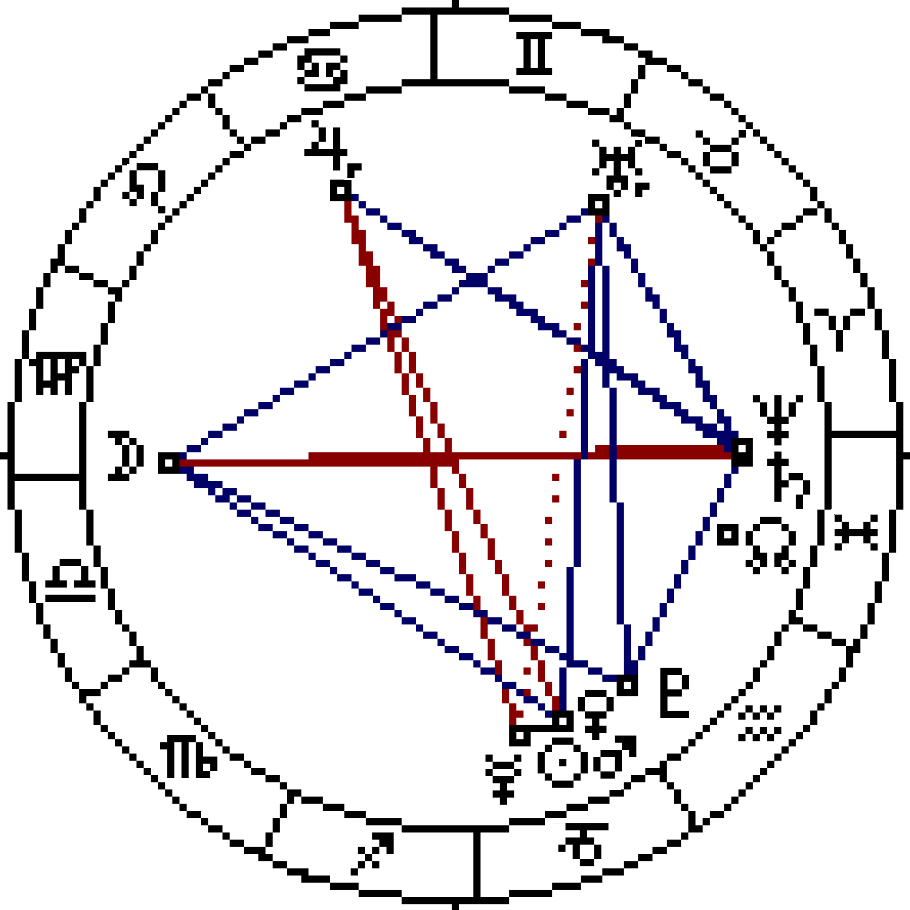
\includegraphics[scale=0.085]{i-diamond.png}

\vspace{-30.2mm}
As long as the core idea (or maybe another idea) does not\newline
return to a state where it appears to be clearly a major\newline
discovery regarding the nature of life and the world\newline
in a way that has not even been considered by others\newline
in the past, additional publications would at most proceed\newline
very, very leisurely, as hobbies on the side, if and only if\newline
they feel like it to me personally for my own felt pleasure.

I have done a lot to interest others into my findings since 2002,
way more than absolutely necessary,
and have taken care to preserve my works at least threefold last year
(2025 book, full website to Usenet, web source to GitHub).

As long as I cannot recover the core idea
and nobody really reacts to any of my ideas and findings,
I estimate that things will at most evolve very, very slowly,
which is not necessarily bad,
maybe more likely even the contrary…

{\color{xphi}I guess,
I am simply the \textbf{guardian lion},
not in the sense of protecting\hspace{0.05em}—\hspace{0.05em}%
that is handled effortlessly by something else\hspace{0.05em}—\hspace{0.05em}%
just keeping the garden intact\,…}
{\color{darkgray}\tiny 25 Jan}

Published a new idea/\hspace{0.03em}hypothesis
that life and awareness/consciousness would be one and the same,
namely the process by which life locally reduces entropy
while exporting the excess entropy into the environment,
with maybe even a relation to measurement and path integrals in quantum mechanics\,…
{\color{darkgray}\tiny 29 Jan}

Sleeping Beauty Dreaming of \ELEMENTAL\,…
{\color{darkgray}\tiny 5 Feb}

I was unaware that 8 January early in the evening was a retrograde Jupiter return,
while I was aware that 25 January was Neptune very late in Pisces,
like at its station in 2024,
and 5 February was my anticipated third Saturn return of the second cycle,
the one to be effective for the next 29 years,
with houses similar to my birth.
%
Just one second after the return,
I heard a church bell just once,
which reminded me also of how Jack Kerouac’s \textsl{Big Sur} begins,
I guess the bell was 7 seconds late for 4:15 PM in Adliswil,
and Saturn then “asked me” how stupid I was
after “asking” whether to publish the series of pocket books
in the hope of reaching my contemporaries,
effectively just recommending to do nothing.
%
I am still maybe hoping for the next Jupiter return in May,
while I guess 
\includegraphics[scale=0.05]{i-jackdaw.jpg}’s \ELEMENTAL\
would have been recommended by Saturn,
also since akin to \textsl{time} via Cronos/Chronos in Greek mythology
and the seventh astrological planet.

I guess all of this does not exclude me writing additional books
like an {\color{gray}exactphilosophy.net series} of pocket books,
each tome reduced to a single theme without distracting anecdotes,
while any hopes that active promotion would be helpful would be more than in vain,
would be outright stupid.
%
Should collective interests change in the rest of my lifetime,
people would come and discover by themselves,
while I estimate that to be rather unlikely.
%
And as a statement and also for research,
\ELEMENTAL\ seems more fruitful,
just one saturnian small thing.
%
And I am also curious about my next Jupiter return 10 May,
curious what might maybe grow from it then,
as hope in a way never dies.

Once more,
like the article \href{https://www.exactphilosophy.net/renegades.pdf}{\color{xphi}\textsl{Renegades}} last year,
not the typical minimal enumeration of what I did relative to this website on this page,
but I guess it was necessary,
and even is to keep this right here this time.

One more thing:
Seven was also the number of Apollon,
while six was the number of Artemis,
with asteroid 105 Artemis just ahead of Saturn at my return,
I guess another hint at Sleeping Beauty Dreaming of \ELEMENTAL\,…

Article \href{https://www.exactphilosophy.net/life-is-awareness.pdf}{\color{xphi}\textsl{Life is awareness\,?}},
and maybe more on coming pages in time.

Published first free online pdf
of the {\color{gray}exactphilosophy.net series}
of pocket books (with just covers+preface).
%
The ancient Greek saying that the beginning is half of the whole
implies maybe also that it is not only important what you begin
but also when you do so.
%
First time online Friday 13 February 2026 at 19:53 CET.

I guess and hope that this series will be a beautiful addition
to the lives of many readers in the future,
while I am at my core more avantgarde,
hence the series would likely become
what I do daily when no longer writing software for a living,
while research and maybe posting,
and hopefully \ELEMENTAL,
would be part of my hobbies then%
\hspace{0.05em}—\hspace{0.05em}%
the three Fates willing, of course\,…

For the time being,
except the first tome with core web as appendix,
I aim to focus on tomes in english only,
for manifold reasons
and especially because translation to almost any language
will likely become ubiquitous in the near future.

Or the series will just grow symmetrically,
maybe even more likely.

It seems that the purely hypothetical “transpluto” dubbed “Isis”
would have had more influence on my life
than I would have anticipated,
see my birth chart and the ones of my parents,
or also the one of Robert Graves,
the author of the \textsl{The White Goddess}.
%
This seems to imply
that likely astrology would be even more detached
from actual planets and stars
than I would have expected,
not because the object is hypothetical
but because it is not widely known.
%
16 February.

(This could, of course,
have been just a “coincidence” so far,
but reminds already more of a “habit”
as in the anecdote that Robert Graves used in a talk
that is reproduced at the end of the 1997 edition of \hspace{-0.05em}\textsl{The White Goddess}
and remember Isis appearing to Lucius at the end of Apuleius’ \hspace{-0.1em}\textsl{The Golden Ass}.
%
Would seem to relate quite a bit
to at least one core aspect of my research and life.)

Asked my Sabian Symbols oracle for tips/help regarding only english or bilingual:
VIRGO 3 Two angels bringing protection.
KEYWORD:  Security.
%
I guess is maybe the moon in Libra
at the tail of the dragon aspect figure
of my currently active Saturn return
since about two weeks.
%
What about the return of the fire horse\,?

I guess rationally is better to have two lanes for a books series,
even though the german ones would be secondary,
would often be using idioms from the english originals,
but maybe nobody will care.
%
Growth would be slower and quite a bit more work.
%
But do I want to grow quickly\,?
%
Rather do more research
and maybe then be better able to describe things
and even \ELEMENTAL\,?
%
Maybe I should just trust that things will turn out well for the time being l,
even if I do not fully understand how and why that could be.
%
Nobody is reading this now anyways.

As long as there is no real feedback to my work,
my “obligations” are essentially towards the future,
way more likely even beyond my own tiny lifetime.

I have decided to make the core website english only again.
%
In other words, remove the core web in german,
and there will also be no {\color{gray}exactphilosophy.net series} in german
except maybe much later;
what will remain are the articles in german under \cometartemis.
%
Reasons are manifold, including that too much work to maintain symmetric,
discoveries thus far not fundamental enough for extra effort
(appeared differently when I created the german version),
translation from english to almost any language will likely be ubiquitous in the relatively near future,
not only for digital documents, also for printed ones,
and more and more people can read and understand basic english quite well,
and so on.
%
In the end is a decision of the heart,
not lightly taken,
of course.
%
I will preserve the current web as web2026.zip,
see the article \textsl{Web archives},
and will likely extract two pages of the timeline into an other document.
%
19 Feb 2026 around 18:45 CET.

\end{itemize}
\normalsize

\noindent
Especially the last paragraph was only very briefly online at the time,
removed again the same evening,
but it reflects the ambivalence of this all.

As it looks now,
at the very end of winter,
Friday 20 March 2026 around noon,
the core web will remain in English and German,
and the German version will likely even be refined,
even though I could never make up for all the time
that went into the English version since at least 2005.
%
The {\color{gray}exactphilosophy.net series} of pocket books
will also keep a symmetric setup,
may well grow in both languages in parallel.
%
That does not exclude sometime in the future to stop doing things in parallel
while then making sure that the German stuff would be appropriately published
and archived outside of my private sphere.

As I noticed two days ago,
the Swiss National Library has actually already archived my website 3 times since December 2021,
including the noindex stuff (except not all images)
and except zip files and stuff linked only from pdfs,
which is fine.
%
Three is the number of Fates.
%
Similarly,
or maybe rather “destiny”,
with Sedna in Gemini (“twin site, twin books”),
the moon in early Libra (“balance of two”) in my current Saturn return for the coming 29 years,
and maybe generally an “Isis” theme in my life,
writing in parallel in English and German could well be destiny,
at least for as long as I am fit enough to do both in parallel.

But \ELEMENTAL,
for all that it appears,
will grow only in very short and simple English,
and I would likely never translate it or permit translations in my lifetime,
except “never say never”, of course:
If many people showed interest,
for example,
I would not deprive them from that.
%
As it emerged after 10 March with switching from XeLaTeX to LuaLaTeX/Node,
for good 17 March when I got two new test prints and they also looked great on paper,
using something with “lua” (moon in Portuguese) did make the visual output rounder and smoother,
even though even when rasterized at 600 dpi in Photoshop it was hard to see differences.
%
That would,
of course,
arguably mirror my moon at my MC.

Finally,
I will almost certainly continue to do research,
and I hope that I was able to catch a tiny bit of the “free absolutum”
released by this Neptune-Saturn “quantum carburetor”
(
\includegraphics[scale=0.034]{i-neptune}\hspace{0.1em}
\includegraphics[scale=0.03]{i-saturn} $\sim\Psi\hbar$)
with their entries into Aries,
namely the ideas about life as awareness
and maybe also hypothetical “Transpluto” Isis.

But things could change again.
%
For example,
for now I am also intending to keep hosting this website on its Raspberry Pi Zero 2 W,
even thought it occasionally crashes for no clear reason,
seems not to overheat,
except maybe the SD card,
but that one is industrial grade.
%
I presume this is related to the “Kyoto Zen Garden” allegory because,
as my parents told me,
in Japan people often even introduce small errors
(or at least did so in the past)
because only gods/goddesses are perfect.
%
Similarly,
with LuaLaTeX/Node,
the page numbers do not iterate through the 9 different glyphs per number in my Jackwrite font,
yielding a slightly less realistic simulation of a physical typewriter.

Wei Chi, but if the little fox\,…
\,\raisebox{-0.3em}{
\includegraphics[scale=0.008]{i-foxyfox.jpg}}

\begin{center}
{\footnotesize\color{xphi}\ \ \ $\pi$: Let x$\varphi$ be; do other things, incl.\ research and write \ELEMENTAL.\newline Lean back, people might still come and see.\par}
\end{center}

\end{document}